\chapter{Introduction}\label{ch:introduction}

\setlength{\epigraphwidth}{0.85\textwidth}
\epigraph{``There is a race between the increasing complexity of the systems we build and our ability to develop intellectual tools for understanding their complexity. If the race is won by our tools, then systems will eventually become easier to use and more reliable. If not, they will continue to become harder to use and less reliable for all but a relatively small set of common tasks. Given how hard thinking is, if those intellectual tools are to succeed, they will have to substitute calculation for thought.''}{\begin{flushright}--Leslie \citet{lamport2002discussion}, \href{https://www.microsoft.com/en-us/research/uploads/prod/2016/12/A-Discussion-With-Leslie-Lamport.pdf}{\textit{A Discussion with Leslie Lamport}}\end{flushright}}

Computational complexity is of such concern in computer science that a great deal of the field is dedicated to understanding it through the lens of function analysis and information theory. In software engineering, researchers are primarily interested in the complexity of building software -- the digital manifestation of algorithms on physical hardware. One kind of software complexity is the cognitive effort required to understand a program.\hspace{-.08em}\footnote{This can be approximated by various metrics like cyclomatic or Halstead complexity.} While today's software is becoming rapidly more intelligent, it shows few signs of becoming more intelligible. Better tools are needed for managing the complexity of building software systems.

\textit{The objective of this thesis is to develop methods that reduce the cognitive effort required to build intelligent systems, using developer tools, programming language abstractions, automated testing, and virtualization technology.}

Broadly speaking, intelligent systems differ from ordinary software systems in that they enable machines to detect patterns, perform tasks, and solve problems which they are not explicitly programmed to solve and which human experts were previously incapable of solving by hard-coding explicit rules. Typically, these systems are able to:\\
%
\begin{enumerate}
    \item learn generalizable rules by processing large amounts of data
    \item tune a large number of free parameters (thousands to billions)
    \item outperform well-trained humans in domain-specific tasks
\end{enumerate}
%
While the idea of intelligent systems has existed for decades, three critical developments made modern intelligent systems ultimately successful. First, computer processing power has become faster, cheaper, and much more readily available. Similarly, the digitalization of new datasets has made vast amounts of information available, and data storage costs have plummeted dramatically. (A \$5 thumb drive today has 200 times more storage capacity than a 2,000 pound, 5 MB, IBM hard drive that leased for \$3,000 per month in 1956.) Most importantly, has been the development of more efficient learning algorithms.

In recent years, computer science and software engineering has made significant strides in building and deploying intelligent systems. Nearly every mobile computer in the world is able to detect objects in images, perform speech-to-text and language translation. These breakthroughs were the direct result of fundamental progress in neural networks and representation learning. Also key to the success of modern intelligent systems was the adoption of collaborative open source practices, pioneered by the software engineering community. Software engineers developed automatic differentiation libraries like Theano~\citep{bergstra2010theano}, Torch~\citep{collobert2002torch} and Caffe~\citep{jia2014caffe}, and built many popular simulators for reinforcement learning. The ease of use and availability of these tools was crucial for democratizing deep learning techniques.

Intelligent systems are widely deployed in virtual settings like data science and cloud services. But even with the tremendous success of machine learning algorithms in fully-observable domains like image recognition and speech processing, intelligent systems have yet to be widely adopted in robotics (at the time of writing this thesis). This dilemma can be partly attributed to various theoretical problems such as domain adaption and transfer learning. Yet with the proven capabilities of modern learning algorithms, exponential increase in processing power, and decades-long effort in building physically-embodied intelligent agents, we should have more progress to show. Why has this goal evaded researchers for so long? One reason, we conjecture, is a lack of programming tools and abstractions for designing, developing, deploying and evaluating intelligent systems. In practice, these activities consume a large amount of cognitive effort without the right set of tools and abstractions.

In traditional software engineering, the Waterfall model (\autoref{fig:waterfall_model}) is a classical model for software development consisting of various stages~\citep{royce1987managing}. We propose contributions to four stages: First, we demonstrate an integrated development environment for \textit{designing} robotics software (\autoref{ch:hatchery}). Next, we show a type-safe domain-specific language for \textit{implementing} differentiable programs, an emerging paradigm in deep learning (\autoref{ch:kotlingrad}). To \textit{verify} this application, we use a set of techniques borrowed from property-based testing~\citep{fink1997property} and adversarial learning~\citep{lowd2005adversarial} (\autoref{ch:difftest}). Docker containers~\citep{merkel2014docker} are used to automate the \textit{maintenance} of reproducible robotics applications on heterogeneous hardware platforms (\autoref{ch:ducker}). Finally, we offer some concluding remarks and lessons learned building these tools in (\autoref{ch:conclusion}).

\begin{figure}[H]
    \centering
    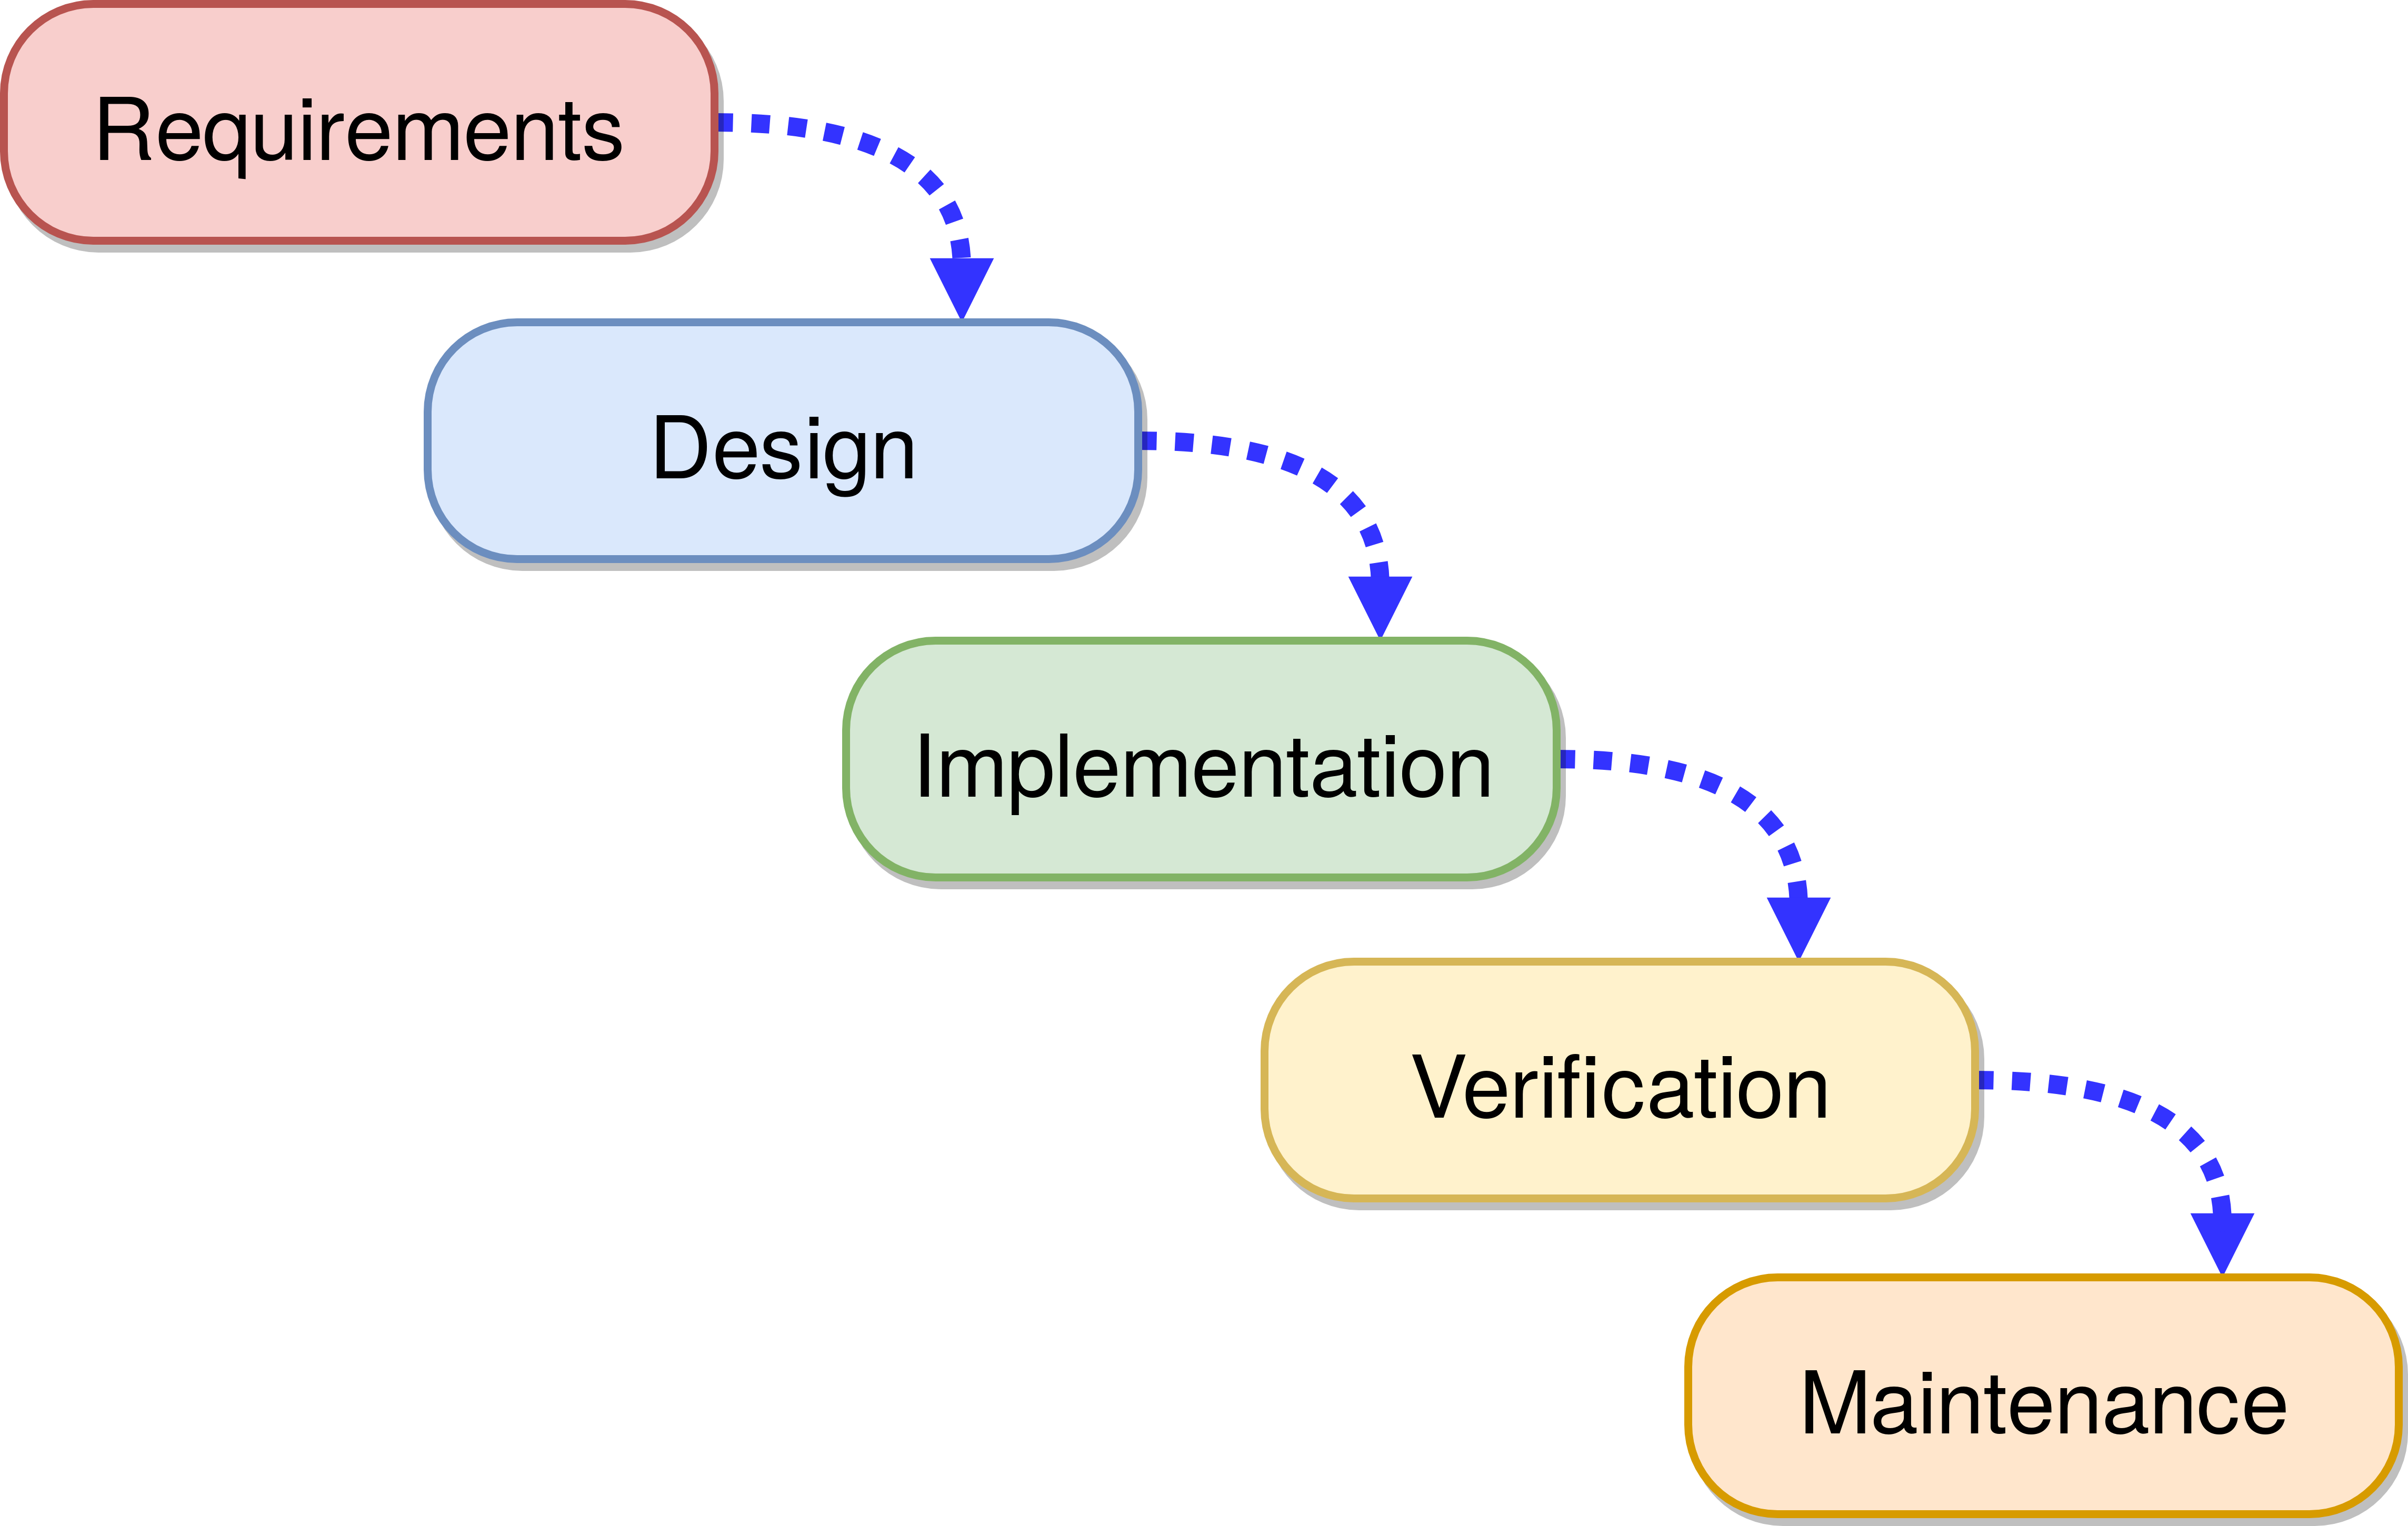
\includegraphics[width=0.70\textwidth]{../figures/waterfall_diagram.png}
    \caption{Royce's original waterfall model describes the software development process. We use it to guide our discussion and frame our contributions inside of this model.\vspace{-10pt}}
    \label{fig:waterfall_model}
\end{figure}

\section{Design: Programming tools for robotics}

Today's software systems are deeply complex entities. Gone are the days where a solitary programmer, even a very skilled one, could maintain a large software system alone. To effectively scale modern software systems, programmers must pool their mental capacity to form a knowledge graph. Software projects which rely on a small set of maintainers tend to perish due to the so-called \textit{bus factor}~\citep{cosentino2015assessing} -- large portions of the knowledge graph are locked inside someone's head. Successful software projects learn how to distribute this graph and form connections to the outside world. The knowledge graph which accumulates around a software project contains facts, but it also contains workflows for programming, debugging, and delivery -- common paths through the labyrinth of software development~\citep{naur1985programming}. Components of this graph can be committed to writing, but documentation is time-consuming and grows stale over time. What is needed is a system that offers the benefits of documentation without the burdens of maintenance.

The development of software systems has a second component, the social graph. The social graph of a successful software project contains product designers, managers and software engineers who work in concert to build software that is well-designed, cohesive, and highly performant. Sometimes this means revising the specification to accommodate engineering challenges, or rewriting source code to remove technical debt. Software design is a multi-objective optimization process and requires contributors with a broad set of skills and common set of goals. To produce software that approximates the criteria of its stakeholders, developers are asked to provide rapid prototypes, and continuously integrate user feedback. Yet today's software systems are larger and more unwieldy than ever. So finding ways to collaborate more effectively is critical to building more intelligent systems.

First, let us consider the mechanical process of writing software with a keyboard.

Integrated development environments (IDEs) can assist developers building complex software applications by automating certain repetitive programming tasks. For example, IDEs perform static analyses and inspections for catching bugs quickly. They provide completion, refactoring and source code navigation, and they automate the process of building, running and debugging programs. While these tasks may seem trivial, their automation promises increased developer productivity by delivering earlier feedback, detecting clerical errors, and freeing mental resources to be used elsewhere. Rather than being forced to concentrate on the structure and organization of text, if developers are able to manipulate code at a semantic level, they will be much happier and more productive. Furthermore, by automating mechanical tasks in software development, these tools free one's attention towards the fundamental activity of writing and understanding programs.

But what are IDEs really doing? They are guiding developers through the knowledge graph of a software project. Consider what a new developer must learn to get up to speed: in addition to learning the language, developers must learn to use libraries and frameworks (arguably languages in their own right). They must become familiar with command line tools for software development, from build tools to version control and continuous integration. They must become familiar with the software ecosystem, programming styles, conventions and development workflows. And they must learn how to collaborate on a distributed team of developers. By automating common tasks in an interactive programming environment and making the graph connectivity explicit through document markup~\citep{goldfarb1981generalized} and projectional editing~\citep{voelter2014towards}, a well-designed IDE is a tool for graph traversal. It should come as little surprise IDEs are really graph databases.

In some aspects, the development of intelligent systems is no different than classical software engineering. The same principles and best-practices which guide software engineering are also applicable to intelligent systems. And the same activities, from design to maintenance will continue to play an important role in building intelligent systems. But in other respects, the generic programming tools used to develop traditional software will require domain-specific adaptations for learning systems to become truly first-class citizens in the next generation of intelligent software, particularly in the case of robotics development.

Towards that goal, we developed an IDE for the \href{https://www.ros.org/}{Robot Operating System} (ROS) called \href{https://github.com/duckietown/hatchery}{Hatchery}. It supports a number of common workflows for ROS development, such as creating ROS nodes, Gazebo simulator integration, support for remote debugging, static analysis, autocompletion and refactoring. In \autoref{ch:hatchery} we discuss the implementation of these features and some of the challenges of building language support, programming tools and integrating with the ROS middleware. We argue that such tools reduce the cognitive complexity of building ROS applications by adopting explicit coding conventions, annotating unstructured text and automating repetitive development tasks.

\section{Implementation: Type-safe differentiable programming}

In the early days of machine learning, it was widely believed that human-level intelligence would emerge from a sufficiently descriptive first-order logic. By accumulating a database of facts and their relations, researchers believed they could use symbolic reasoning to bypass learning altogether. This rule-based approach dominated a large portion of early research in artificial intelligence and considerable effort was poured into the creation of domain-specific ontologies to capture human knowledge. Despite the best efforts of roboticists, signal processing engineers and natural language researchers, \textit{expert systems} were unable to scale to real-world applications, causing a great disillusionment in artificial intelligence research for several decades. While computer scientists underestimated the difficulty of \textit{learning}, expert systems excelled in areas where current machine learning systems struggle such as classical reasoning and interpretability, and there is growing evidence to suggest many of these ideas were simply ahead of their time. In our work, we take inspiration from some early work in symbolic reasoning~\citep{dwyer1948symbolic, glushkov1971analitik}, type systems~\citep{lof1973intuitionistic,jay1996shape} and functional programming~\citep{mccarthy1960recursive, abelson1996structure}.

What was finally shown to scale, is the idea of connectionist learning. By nesting random function approximators, called perceptrons, and updating the free parameters using backpropagation~\citep{werbos1990backpropagation, rumelhart1988learning}, the resulting system is capable of learning a surprising amount of intelligent behavior. The approach, termed artificial neural networks (ANNs), can be traced back to the mid-20th century~\citep{ivakhnenko1965cybernetic, rosenblatt1958perceptron}, but was not fully-realized in silico until after the widespread availability of cheap computing and large datasets~\citep{lecun2015deep}. In theory, a single layer of nesting is able to approximate any continuous differentiable function~\citep{hornik1989multilayer}, but in practice, learning requires composing many such approximators in a deeply nested fashion, hence the term, \textit{deep neural networks} (DNNs). The importance of depth was suspected for many years, but the original backpropagation algorithm had difficulty training DNNs due to the vanishing gradient problem~\citep{bengio1994learning}. Solving this problem required a number of adaptations and many years to fully debug. It was not until circa 2013 when deep learning was competitive with human experts in specific domains.

While it took fundamental research in deep learning to realize the connectionist blueprint, the success of modern deep learning can be partly attributed to software tools for calculating mathematical derivatives, a key step in the backpropagation algorithm. Although it has not yet been established if or how derivatives might be calculated in biological circuits, derivatives are essential for ANN training. For many years, the symbolic form of these derivatives were analytically derived when prototyping a new neural network architecture, a tedious and error-prone process. There is a well-known algorithm in the scientific computing community dating back to the 1970s, called \textit{automatic differentiation} (AD)~\citep{linnainmaa1970representation, griewank1989automatic}, which is able to calculate derivatives for arbitrary differentiable functions. But surprisingly, it was not until much later, after the development of Theano~\citep{bergstra2010theano} when AD became widely adopted in the machine learning community. This library greatly accelerated the pace of deep learning research and spurred the development of other AD frameworks like TensorFlow~\citep{abadi2016tensorflow} and PyTorch~\citep{paszke2019pytorch}.

Engineered intelligent systems must think carefully about languages and abstractions. If developers are to implement backpropagation by hand, they will have scarce time to think about the high-level characteristics of these systems. Similarly, if programming abstractions are too specific, small variations will require costly reimplementation. This is no different from traditional software engineering -- as engineers, we need to choose the right abstractions for the task at hand. Too low-level and the design is lost in the details -- too abstract and the details are lost completely. With deep learning, the necessity of choosing good abstractions is even more important, as the relationship between source code and behavior is already difficult to debug, due to the complexity of neural networks and array programming. One component of that complexity can be found in the type system.

Most existing AD frameworks for machine learning are written in dynamically-typed languages like Python, Lua and JavaScript, with some early implementations including projects like \href{http://deeplearning.net/software/theano/}{Theano}~\citep{bergstra2010theano}, \href{http://torch.ch/}{Torch}~\citep{collobert2002torch} and \href{https://caffe.berkeleyvision.org/}{Caffe}~\citep{jia2014caffe}. Similar ideas have arisen in statically-typed, functional languages, such as Java (\href{https://github.com/uniker9/JAutoDiff}{JAutoDiff}~\citep{nureki2012jautodiff}, \href{https://deeplearning4j.org/}{DL4J}~\citep{team2016dl4j}, \href{https://github.com/Hipparchus-Math/hipparchus}{Hipparchus}~\citep{andrea2016automatic}), Scala (\href{https://tongfei.me/nexus/}{Nexus}~\citep{chen2017typesafe}), F\# (\href{http://diffsharp.github.io/DiffSharp/}{DiffSharp}~\citep{baydin2015diffsharp}), \href{https://www.tensorflow.org/swift}{Swift}~\citep{lattner2018tensorflow}, Haskell (\href{https://github.com/leopiney/tensor-safe}{TensorSafe}~\citep{pineyro2019structure}) et al., but few of these are able to check the shape of multidimensional arrays in their type system, and those which do are implemented in experimental languages with dependent types. In our work, we demonstrate the viability of shape-checking in a widely-used language. This ensures that programs on matrices, if they compile, are the correct shape and can be numerically evaluated at runtime.

\href{https://github.com/breandan/kotlingrad/}{Kotlin$\nabla$} is an embedded domain-specific language (eDSL) for differentiable programming in a language called \href{https://kotlinlang.org}{Kotlin}, a statically-typed programming language with support for asynchronous programming and multi-platform compilation. In Kotlin$\nabla$ (\autoref{ch:kotlingrad}), we describe an algebraically-grounded implementation of automatic differentiation with shape-safe tensor operations. Our approach differs from most existing AD frameworks in that Kotlin$\mathbf{\nabla}$ is the first shape-safe AD library fully compatible with the Java type system, requiring no metaprogramming, reflection or compiler intervention to use.

\section{Verification: Testing intelligent systems}

Most naturally arising phenomena, particularly those related to vision, planning and locomotion are high dimensional creatures. Richard Bellman famously coined this problem as the ``curse of dimensionality''~\citep{bellman1957dynamic}. Our physical universe is populated with problems which are simple to pose, but seemingly impossible to solve inside of it. Claude Shannon, a contemporary of Bellman, calculated the number of unique chess games to exceed $10^{120}$, more than the number of atoms in the universe by approximately forty orders of magnitude~\citep{shannon1950chess}. At the time, it was believed that such problems would be insurmountable without fundamental breakthroughs in algorithms and computing machinery. Indeed, while Bellman or Shannon did not live to see the day, it took only half a century of progress in computer science~\citep{campbell2002deep} before solutions to problems with the same order of complexity, first discovered in the Cambrian explosion 541 million years ago, were implemented to a competitive margin on modern computers~\citep{pratt2015cambrian}.

While computer science has made enormous strides in solving the common cases, Bellman's curse of dimensionality still haunts the long tail of machine learning, particularly for distributions that are highly dispersed. Because the dimensionality of many real-world functions that we would like to approximate is intractably large, it is difficult to verify the behavior of a candidate solution in all regimes, especially in settings where failure is rare but catastrophic. According to some studies, humans drivers average 1.09 fatalities per hundred million miles~\citep{kalra2016driving}. A new software build for an autonomous vehicle would need to accumulate 8.8 billion miles of driving in order to approximate the fatality rate of a human operator to within 20\% with a 95\% confidence interval. Deploying such a scheme in the real-world would be logistically, not to mention ethically, problematic.

Realistically speaking, intelligent systems need better ways to practice their skills and probe the effectiveness of a candidate solution within a limited computational budget, without harming humans in the process. The goal of this testing is to highlight errors, but ultimately to provide feedback to the system. In software engineering, the real system under test are the ecosystem of humans and machines which provide each other's means of subsistence. The success of this arrangement depends on an external testing mechanism to enforce a minimum bar of rigor, typically some form of hardware- or human-in-the-loop testing. If the testing mechanism is not somehow opposed to the system under test, an intelligent system can deceive itself, which is neither in the system's nor its users' best interest.

More broadly, we can view type checking (\autoref{ch:kotlingrad}) and automated testing (\autoref{ch:difftest}) as part of a larger toolset for software verification and validation. The sooner anomalies are detected, the easier they are to fix and the safer autonomous systems can become. Previous automated testing approaches have required considerable domain expertise to successfully deploy, but recent progress in metamorphic testing~\citep{chen1998metamorphic} and self-supervised learning~\citep{lieb2005adaptive} have shown applications in increasingly general domains~\citep{zhang2020testing}. Towards that goal, in \autoref{ch:difftest} we propose a novel algorithm inspired by property-based testing and adversarial learning which empirically improves data efficiency, and requires far less domain expertise to implement than na\"ive property-based methods.

\section{Maintenance: Tools for reproducible robotics}

One of the challenges of building intelligent systems and programming in general, is the problem of reproducibility. Software reproducibility has several challenging aspects, including hardware compatibility, operating systems, file systems, build systems, and runtime determinism. While writing programs and feeding them directly into a computer may have once been common practice, today's source code is far too removed from its mechanical realization to be meaningfully executed in isolation. Today's handwritten programs are like schematics for a traffic light -- built inside a factory, and which require a city's-worth of infrastructure, cars, and traffic laws to serve their intended purpose. Like traffic lights, source code does not exist in a vacuum -- built by compilers, interpreted by virtual machines, executed inside an operating system, and which follow a specific communication protocol -- programs are essentially meaningless abstractions outside this context.

As necessary in any good schematic, much of the information required to build a program is divided into layers of abstraction. Most low-level instructions carried out by a computer during the execution of a program were not written nor intended to be read by the programmer and have since been automated and forgotten. In a modern programming language like Java, C\# or Python, the total information required to run a simple program often numbers in the trillions of bits. A portion of that data pertains to the software for building and running programs, including the build system, software dependencies, and development tools. Part of the data pertains to the operating system, firmware, drivers, and embedded software. For most programs, such as those found in a typical GitHub repository, a vanishingly small fraction of the information corresponds to the source code itself.

Applied machine learning shares many of the same practical challenges as traditional software development, with source code, release and dependency management. The current process of training a deep learning model can be seen as particularly long compilation step, but it differs significantly in that the source code is a high-level language which does not directly describe the computation being performed, but is a kind of meta-meta-program. The first meta-program describes the connectivity of a large directed graph (i.e.~ a computation graph or probabilistic graphical model), parameterized by weights and biases. The tuning of those parameters is another meta-program, describing the sequence of operations required to approximate a program which we do not have access, save for some input-output examples. Emerging techniques in meta-learning and hyper-parameter optimization (e.g.~differentiable architecture search~\citep{liu2018darts}) add even further meta-programming layers to this stack, by searching over the space of directed graphs themselves.

Hardware manufacturers have developed a variety of specialized accelerators to train and run these programs rapidly. But unlike most programming, deep learning is a much simpler model of computation -- so long as a computer can add and multiply, it has the ability to run a deep neural network. Yet due to the variety of hardware platforms which exist and the software churn associated with them, reproducing deep learning models can be painstakingly difficult on new hardware, even with the same source code and dependencies. Many graph formats, or \textit{intermediate representations} (IRs) in compiler parlance, promise hardware portability but if developers are not careful, their models may not converge during training, or may produce different results on different hardware. Complicating the problem, IRs are produced by competing vendors, selling competing chips with incompatible standards (e.g. MLIR~\citep{mlir}, ONNX~\citep{bai2019}, nGraph~\citep{cyphers2018intel}, Glow~\citep{rotem2018glow}, TVM~\citep{tvm2018} et al.) While some have tried to leverage existing compilers such as GHC~\citep{elliott2018simple} or DLVM/LLVM~\citep{wei2017dlvm}, there are few signs of broader interoperability at the time of writing this thesis.

At the end of the day, researchers need to reproduce the work of other researchers, but the mental effort of re-implementing basic abstractions can impede scientific progress. Tools which facilitate software reproducibility and incremental development are essential. Fortunately, this is the same problem which has concerned the software industry for many years and produced a variety of version control systems (VCS). But VCS alone is insufficient, since these tools are primarily intended to store text. Text-based representations are temporarily stable, but when dependencies are updated and rebuilt, important details about the original development environment can be misplaced. To reproduce a program in its entirety, a snapshot of all digital information available during execution, and ideally, the physical computer itself is needed. Short of a full snapshot, the minimal set of dependencies and a near physical replica is highly desirable. Any variability in the physical or digital dependency graph can be a source of discrepancies which requires time and energy to later isolate.

In order to mitigate the effects of software variability and assist the development of intelligent systems on heterogeneous platforms, we use a developer tool called \href{https://www.docker.com}{Docker}, part of a loosely-related set of tools for build automation and developer operations which we shall refer to as \textit{container infrastructure}. Docker allows developers to freeze a software application and its host environment, allowing developers (e.g.~using a different environment) to quickly reproduce these applications. Docker itself is a technical solution, but also encompasses a set of best-practices and guidelines which are more methodological in nature. While Docker does not address the incompatibility of vendor standards and hardware drivers, it makes these variables explicit, and reduces the difficulty of reproducing software artifacts.

There is a second component to software reproducibility of intelligent systems, which incorporates the notion of time: simulators. Simulators are used in nearly every engineering discipline to imitate a physical process which may be expensive, dangerous or impractical to bring into reality. For example, simulators are often used to model the dynamics of another instruction set architecture~\citep{bellard2005qemu}, the dynamics of electromagnetic transients~\citep{tavante2018opensi}, the dynamics of orbital motion~\citep{bellman1965wengert}, the dynamics of human transportation systems~\citep{ruch2018amodeus}, or the dynamics of driving~\citep{gym_duckietown}. Today's computers are capable of running increasingly high fidelity simulations, but most practitioners agree that simulation alone will never be enough to capture the full distribution of real-world data. In this view, simulation can be a useful tool for detecting errors, but it cannot fully reproduce all the subtleties of the real-world, and should not be a surrogate for testing on real-world data. Others have suggested a middle road~\citep{bousmalis2018using}, where judicious use of simulator training, alongside domain adaptation is a sufficiently rigorous environment for evaluating intelligent systems. Regardless of which view prevails, our goal is to provide rapid feedback to developers, and to make the entire process from testing to deployment as reproducible as possible.

%\subsection{Case study: An application for autonomous robotics}\label{subsec:case-study}
%
%All great software has a secret recipe: software gets better when its authors use the product. In the best case, the authors are the core users -- ideally by choice, if not by necessity. When software engineers are using their own software on a regular basis -- bumping into sharp corners and encountering edge cases firsthand -- the product gets better. When there is an obviously missing feature, it gets implemented. When there is a bug, it gets fixed. It may not be easy to find users who are so inclined, or to build software which is so useful, but there must be some overlap in order for good software to become great. Termed ``dogfooding''~\citep{harrison2006eating}, this practice is an effective mechanism for building self-improving cybernetic systems and an important principle for open source software and safety-critical systems. Putting this principle into practice, we, as the authors and primary users of these tools, validate their effectiveness by developing a robotics application within an IDE (\autoref{ch:hatchery}), containing Kotlin$\nabla$ code (\autoref{ch:kotlingrad}), tested using adversarial fuzz testing (\autoref{ch:difftest}), and which is built and maintained using the Docker stack (\autoref{ch:ducker}).

\section{Contributions}

%Archeologists have been able to trace tool use back millions of years, to the very birth of human civilization. Next to language, tool use is regarded as the Promethean moment in our own evolutionary history and a beacon for the awakening of yet other intelligent species under the sea~\citep{finn2009defensive, mann2013tool}, on the savannas~\citep{chevalier1993tool}, among the treetops~\citep{bertagnolio1994tool}, and perhaps higher still~\citep{kaplan1981astroengineering, carrigan2012interstellar}. Psychologists have only begun to understand the role of infant tool use in the motor development~\citep{adolph2007motor} of humans and other primates~\citep{hayashi2003cognitive, keller2016orangutans}. Inspired by developmental psychology~\citep{min2016affordance}, some roboticists are now studying tool use in the context of affordance learning~\citep{stoytchev2005behavior,sinapov2007learning} and intrinsic motivation~\citep{forestier2016curiosity} in autonomous agents.
%
%\begin{figure}
%    \centering
%    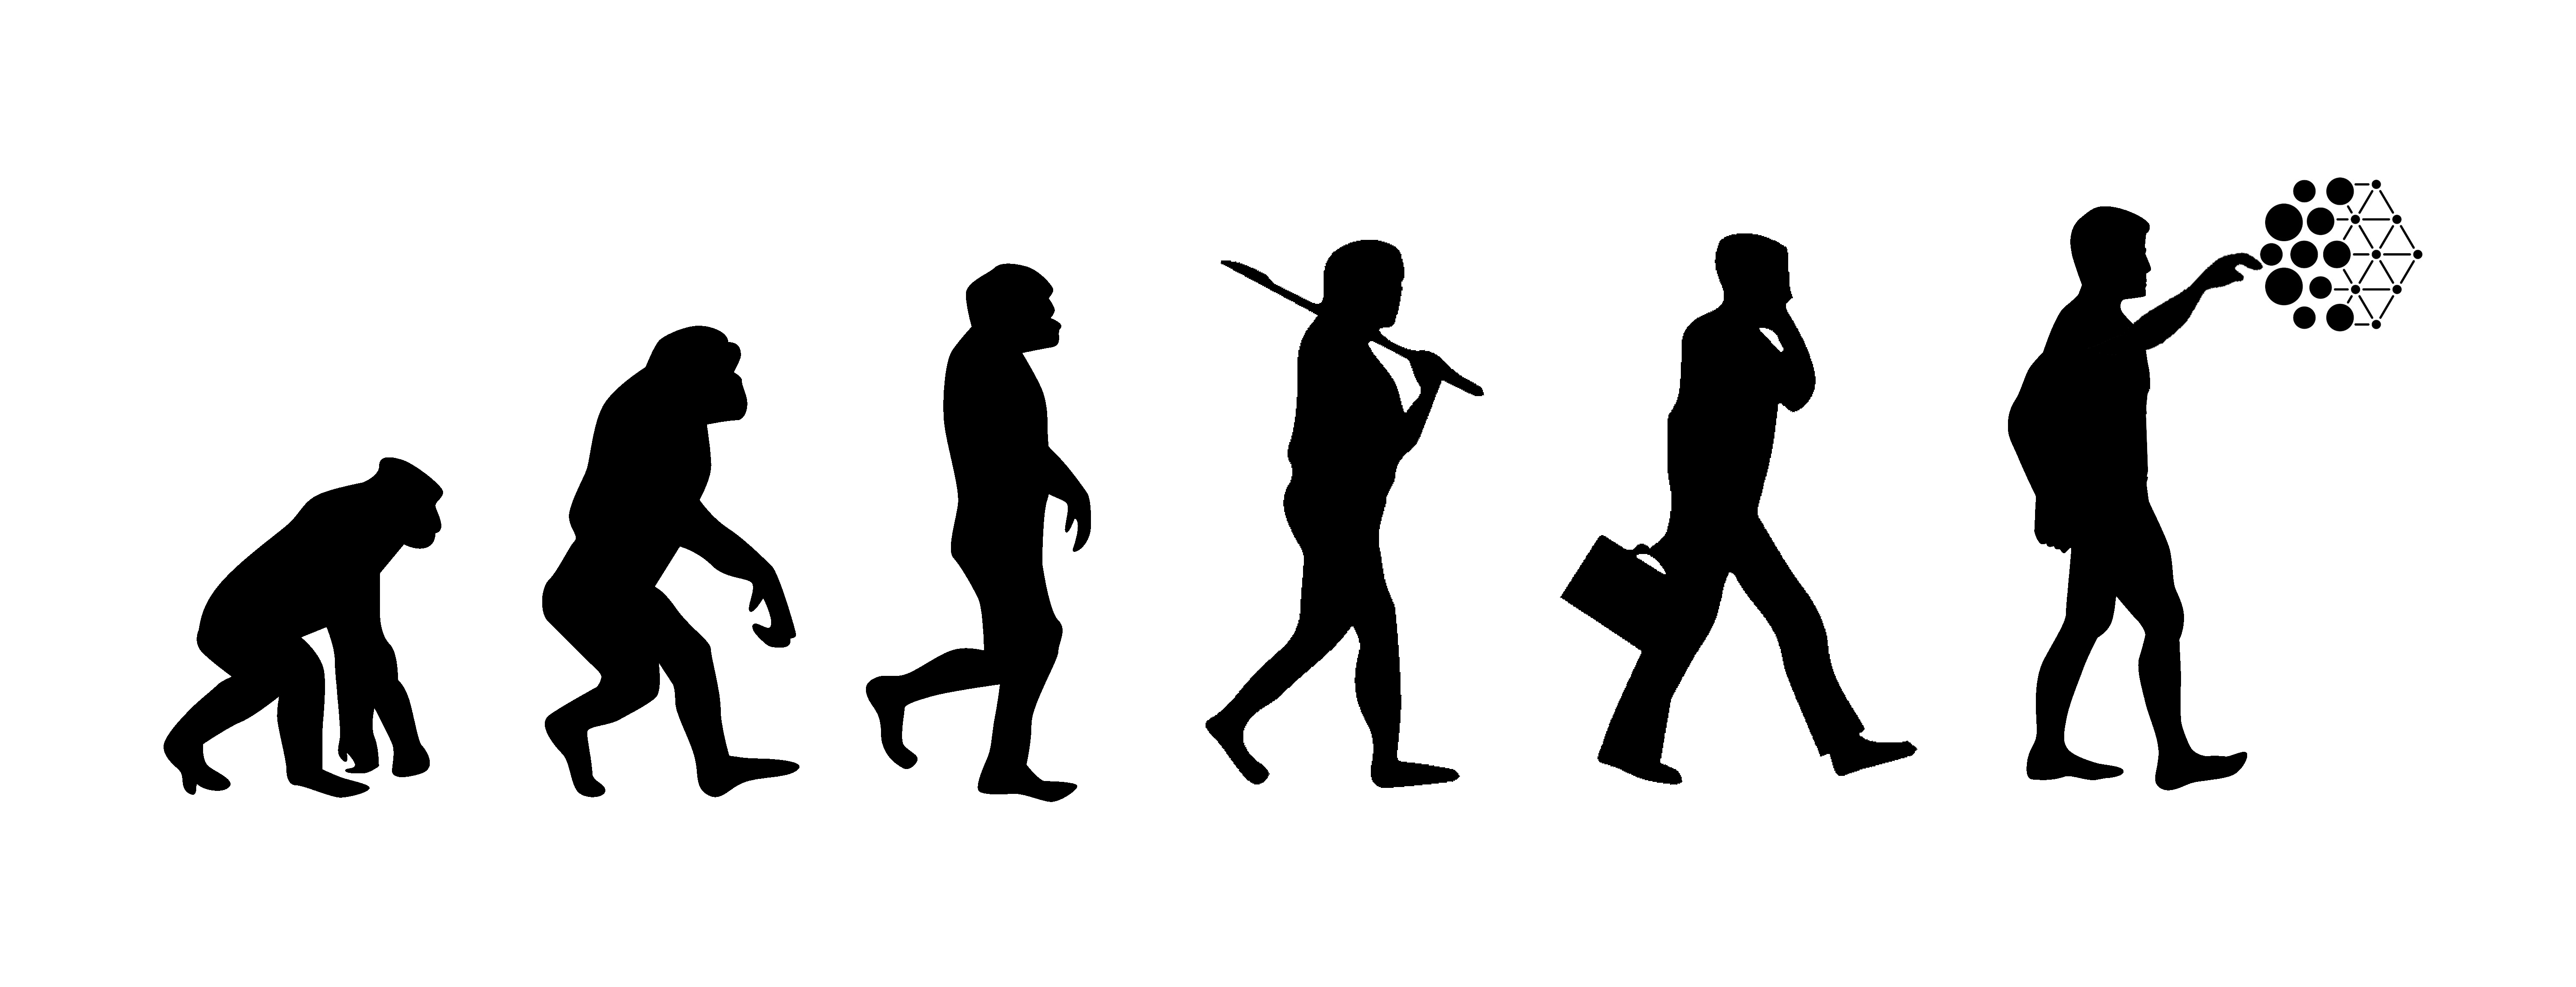
\includegraphics[width=0.90\textwidth]{../figures/evolution.png}
%    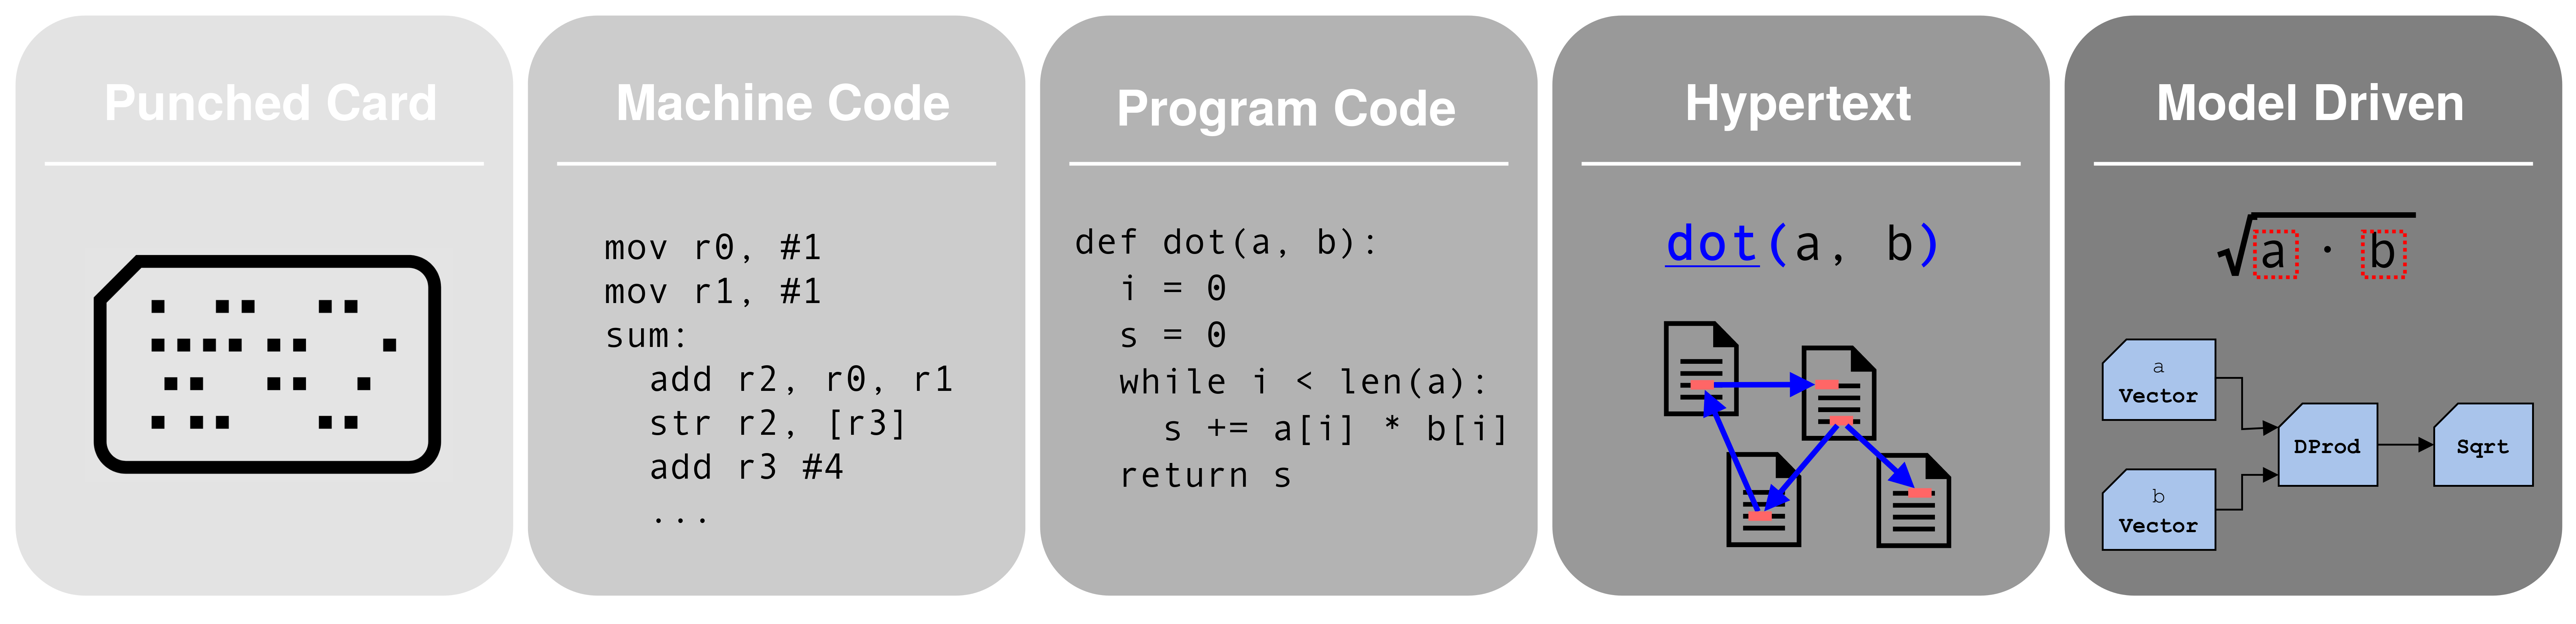
\includegraphics[width=0.90\textwidth]{../figures/progress_in_program.png}
%    \caption{The evolution of code. On the left are languages that force the user to adapt to the machine. To the right are increasingly flexible representations of source code.}
%    \label{fig:evolution_of_programming}
%\end{figure}
%
%With the dawn of the information age, our species is on the brink of a new adolescent era. The same organs once evolved for motion planning in Euclidean configuration space are being employed in ways never dreamt by our progenitors. In this era, one lifetime and the brightest minds of our generation are barely enough to penetrate the boundaries of human knowledge. Engineers must spend the first half of their intellectual careers on knowledge acquisition. Scientists toil for years to build infrastructure needed to run simple experiments. If we are to sprout higher branches from our tree of knowledge, send taproots into deeper wells of understanding, nature's endowments can only carry us so far. If humankind is to reach its full potential in the time we are allotted, its growing population of knowledge workers will need a new toolset to transcend the rising complexity of innovation.
%
%Each step of the knowledge creation process is fraught with incidental complexity arising from the acquisition and mastery of domain-specific expertise, the discovery and transfer of existing knowledge, the design and prototyping process, the validation and verification of those designs, and finally the upkeep and operational aspects of putting knowledge systems into production. This whole enterprise requires an enormous amount of human resources to effectively choreograph. In the information industry, these individuals are often called \textit{architects}, \textit{engineers}, \textit{developers}, \textit{programmers}, or simply \textit{coders}.\footnote{Conflate any of these camps and they will surely protest, but the differences are mostly exaggerated.} According to some surveys~\citep{data2018global}, their population is projected to exceed 61 million by 2020, not to mention the management and administration of their activities in the workplace.
%
\citet{kernighan1976software} first introduce the term \textit{software tools} in the context of Unix command line utilities, roughly in the same spirit as tools this thesis proposes. \citet{thrun2000towards, erez2015simulation} develop language and simulation based tools for robotics development along the same lines. Broadly, we consider any software which assists users engaged in the activity of writing computer programs, as a \textit{programming tool}.

In this thesis we take small steps towards reducing the complexity of programming intelligent systems, through programming tools. First, we show a plugin for building robotics applications (\autoref{ch:hatchery}). Next, we describe a domain specific language for writing differentiable programs (\autoref{ch:kotlingrad}). Using our DSL (\autoref{ch:difftest}) as a vehicle, we develop an adversarial framework for testing differentiable programs and empirically demonstrate its efficiency compared to a probabilistic sampling method. We then discuss a container-based solution for reproducing robotics programs, and more broadly any embedded software system with visuomotor capabilities (\autoref{ch:ducker}). Finally, in \autoref{ch:conclusion} we offer some reflections and predictions for the future of intelligent systems programming. Much work remains on the road ahead. We believe the future is bright and hope those devoted to building it will take some inspiration from the directions proposed herein.

\clearpage

\section{Iconography}

Throughout this thesis, the following iconography is used to denote: \\
%
\begin{enumerate}
    \vspace{-0.2cm}\item[] \inlineimg{../figures/laptop_icon.png} &  Shell commands intended for a personal computer, or output derived thereof. \\
    \vspace{-0.2cm}\item[] \inlineimg{../figures/bnf_file.png} & GrammarKit's \inline{.bnf} parsing expression grammar (PEG)~\footnote{GrammarKit usage notes: \url{https://github.com/JetBrains/Grammar-Kit/blob/master/HOWTO.md}} \\
    \vspace{-0.2cm}\item[] \inlineimg{../figures/docker_icon.jpg} &  Either \inline{Dockerfile}~\footnote{Dockerfile reference: \url{https://docs.docker.com/engine/reference/builder/}} or Docker Compose~\footnote{Compose file reference: \url{https://docs.docker.com/compose/compose-file/}} syntax. \\
    \vspace{-0.2cm}\item[] \inlineimg{../figures/raspi_icon.png}  &  Shell commands which should be run on a Raspberry Pi.\hspace{-.08em}\footnote{Raspberry Pi: \url{https://www.raspberrypi.org/}} \\
    \vspace{-0.2cm}\item[] \inlineimg{../figures/duckietown.png}  &  Duckietown Shell (\inline{dts}) commands.\hspace{-.08em}\footnote{Duckietown Shell: \url{https://github.com/duckietown/duckietown-shell-commands}} \\
    \vspace{-0.2cm}\item[] \inlineimg{../figures/launch_icon.png}  &  roslaunch \inline{.launch} files.\hspace{-.08em}\footnote{ROS Launch XML: \url{https://wiki.ros.org/roslaunch/XML}} \\
    \vspace{-0.2cm}\item[] \inlineimg{../figures/python_icon.png}  &  Python source code.\hspace{-.08em}\footnote{Python documentation: \url{https://www.python.org/doc/}} \\
    \vspace{-0.2cm}\item[] \inlineimg{../figures/kotlin_file.png}  &  Kotlin source code.\hspace{-.08em}\footnote{Kotlin documentation: \url{https://kotlinlang.org/docs/reference/}}
\end{enumerate}